\documentclass[11pt,letterpaper]{article}
\usepackage[utf8]{inputenc}
\usepackage[T1]{fontenc}
\usepackage{lmodern}
\IfFileExists{spanish.ldf}{\usepackage[spanish,es-nodecimaldot]{babel}}{\usepackage{babel}}
\usepackage[letterpaper,margin=2.5cm]{geometry}
\usepackage{graphicx,booktabs,array,float,microtype,enumitem,amsmath}
\usepackage[table]{xcolor}
\usepackage{caption}
\usepackage[hidelinks]{hyperref}
\urlstyle{same}
\setlength{\parindent}{0pt}
\setlength{\parskip}{6pt}
\renewcommand{\arraystretch}{1.20}
\captionsetup{font=small,labelfont=bf}
\renewcommand{\figurename}{Figura}
\renewcommand{\tablename}{Tabla}
\setlist[itemize]{leftmargin=*,nosep}
\newcommand{\Programa}{Maestría en Inteligencia Artificial}
\newcommand{\Asignatura}{Visión Inteligente}
\newcommand{\Estudiante}{Erick Martín Rodríguez Baeza}
\newcommand{\Matricula}{26ZPM034}
\newcommand{\Docente}{I.MT. Luis Alberto Espejo Ponce}
\newcommand{\FechaEntrega}{25 de noviembre de 2026}
\newcommand{\Lugar}{Zacapoaxtla, Puebla}

\newenvironment{hangparas}[2]{\setlength{\parindent}{0pt}\setlength{\leftskip}{#1}\setlength{\parindent}{-#1}}{}

\newcommand{\Actividad}{Actividades 4.2 y 4.3}
\newcommand{\TituloActividad}{Empaquetado y despliegue del clasificador\\de impulsores y tazones}
\newcommand*{\LigaRepositorio}{}
\begin{document}
\renewcommand{\tablename}{Tabla}
\hypersetup{pageanchor=false}
\begin{titlepage}
\begin{center}
\vspace*{3mm}

\includegraphics[width=62mm]{assets/logo_maestria_simbolo.png}
\vspace{7mm}

{\Large\scshape Instituto Tecnológico Superior de\\[1mm] Zacapoaxtla\par}
\vspace{5mm}

{\large\Programa\par}
\vspace{1mm}

{\large\Asignatura\par}
\vspace{7mm}

{\LARGE\bfseries Unidad 4 -- \Actividad\par}
\vspace{5mm}

{\Large\TituloActividad\par}
\vspace{8mm}

{\small\scshape \Lugar\par}
\end{center}
\vfill
\begin{flushright}
\begin{minipage}{0.58\textwidth}
\raggedleft
\textbf{Docente:}\\\Docente
\vspace{6mm}

\textbf{Estudiante:}\\\Estudiante
\vspace{6mm}

\textbf{Matrícula:}\\\Matricula
\vspace{6mm}

\textbf{Fecha:}\\\FechaEntrega
\end{minipage}
\end{flushright}
\end{titlepage}
\setcounter{page}{1}
\hypersetup{pageanchor=true}


\section*{Objetivo y alcance}
Empaquetar el clasificador de impulsores y tazones para que se pueda ejecutar con las mismas dependencias y los mismos pesos en otro equipo. Se reutiliza ResNet18, entrenada en la actividad 3.3, y se conserva el script de la 4.1. El sistema recibe una imagen recortada de una sola pieza y devuelve la clase elegida junto con su confianza.

\section*{Preparación de la entrega}
El repositorio reúne el modelo, el código, los recortes de prueba y el archivo de dependencias. El \texttt{Dockerfile} parte de Python 3.12, instala PyTorch para CPU y copia al contenedor los archivos que requiere el clasificador. Se comparó la huella SHA-256 de los pesos y del script con la copia de la 4.1. Ambas coinciden.

\section*{Verificación en CPU}
La prueba se realizó en Linux con Python 3.12.14, PyTorch 2.5.1+cpu y tres hilos. Se ejecutó el comando de inferencia con una imagen, un lote de hasta ocho recortes y un flujo con pausas de 0.1 s. Las dos modalidades usaron los mismos 33 recortes de la actividad 3.3.

\begin{table}[H]\centering\small
\begin{tabular}{lrrrr}\toprule
Modo & Imágenes & Proceso (s) & Operación (s) & ms/imagen \\\midrule
Lote & 33 & 0.918 & 0.918 & 27.82 \\
Flujo & 33 & 1.107 & 4.313 & 33.54 \\
\bottomrule\end{tabular}
\caption{Mediciones nativas de CPU en Linux.}
\end{table}

El lote y el flujo coincidieron en 33 predicciones. Se reprodujeron 32 aciertos de 33. El recorte \texttt{1\_008.png}, etiquetado como impulsor, volvió a clasificarse como tazón. Los recortes se reutilizan para comprobar la continuidad del modelo. Una prueba con imágenes nuevas permitiría observar su respuesta fuera de este conjunto.

\begin{figure}[H]\centering
\begin{minipage}{0.35\linewidth}\centering
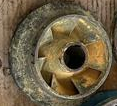
\includegraphics[height=27mm,width=44mm,keepaspectratio]{assets/4_000.png}\par
{\small Impulsor, 95.85\%}
\end{minipage}\hspace{4mm}%
\begin{minipage}{0.35\linewidth}\centering
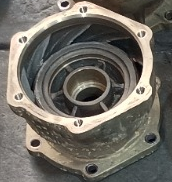
\includegraphics[height=27mm,width=44mm,keepaspectratio]{assets/22_006.png}\par
{\small Tazón, 99.65\%}
\end{minipage}
\caption{Predicciones de dos recortes incluidos y confianza de cada clase.}
\end{figure}

\clearpage
\section*{Ejecución en Docker}
En Windows, abre Docker Desktop y usa contenedores Linux. Ejecuta \texttt{ejecutar\_docker.bat} para construir la imagen y probar el modelo en las dos modalidades. El script guarda una predicción y su confianza para cada fotografía adicional en \texttt{data/propias/}.

\textbf{Estado al preparar esta versión.} El ensayo de Docker está pendiente. Los datos medidos de este reporte corresponden a la ejecución nativa en CPU. La prueba con una foto nueva queda pendiente de contar con esa imagen.


El tiempo de proceso incluye lectura, preparación, inferencia y posprocesamiento. El tiempo de operación en flujo también comprende las pausas. Para repetir la prueba, el README indica los requisitos, el comando y la carpeta donde se guarda la evidencia.

\section*{Entrega del proyecto}
El repositorio permite reconstruir la imagen y contiene el manual de ejecución. El profesor indicó que la imagen construida puede permanecer en el equipo del estudiante. La documentación de las pruebas se presenta por medio del reporte, como alternativa al video (L. A. Espejo Ponce, comunicación personal, 17 de noviembre de 2026).

\ifx\LigaRepositorio\empty
La liga privada se añade tras publicar el proyecto en GitHub.
\else
\href{\LigaRepositorio}{Abrir el repositorio privado de GitHub}.
\fi

\section*{Uso de IA}
Se utilizó ChatGPT como apoyo para organizar el empaquetado, reunir los registros y preparar el reporte. Las cifras de la prueba se obtuvieron al ejecutar el modelo guardado con las imágenes incluidas.

\section*{Referencias}
\small
\begin{hangparas}{0.7cm}{1}
\textit{Cuaderno de trabajo: Unidad IV. Despliegue de un modelo de visión inteligente}. (s. f.). [Material de la asignatura Visión Inteligente].\par
Docker, Inc. (s. f.). \textit{Install Docker Desktop on Windows}. \url{https://docs.docker.com/desktop/setup/install/windows-install/}\par
\end{hangparas}
\end{document}
